\documentclass{article}

% content/resources/templates/preamble.tex
\usepackage[margin=0.6in]{geometry}
\author{Milav Dabgar}
\usepackage{amsmath,amssymb,amsthm}
\usepackage{booktabs}
\usepackage{multirow}
\usepackage{xcolor}
\usepackage{tcolorbox}
\tcbuselibrary{breakable,skins}
\usepackage[colorlinks=true,linkcolor=blue]{hyperref}
\usepackage{titlesec}
\usepackage{enumitem}
\usepackage{tikz}
\usepackage{pgfplots}
\usepackage{circuitikz}
\usepackage[version=4]{mhchem}
\usepackage{longtable}
\usepackage{array}
\usepackage{float}
\usepackage{caption}
\usepackage{listings}

\lstset{
  basicstyle=\small\ttfamily,
  breaklines=true,
  breakatwhitespace=false,
  postbreak=\mbox{\textcolor{red}{$\hookrightarrow$}\space},
  float=false,
  numbers=left,
  numberstyle=\tiny\color{gray},
  numbersep=10pt,
  xleftmargin=2em,
  keywordstyle=\color{blue},
  commentstyle=\color{green!60!black},
  stringstyle=\color{purple},
  backgroundcolor=\color{gray!5},
  showstringspaces=false,
  tabsize=2,
  captionpos=b,
  keepspaces=true,
  columns=flexible
}

\pgfplotsset{compat=1.18}
\usetikzlibrary{shapes,arrows,positioning,calc,patterns,decorations.pathmorphing,decorations.markings,arrows.meta}

% Color scheme
\definecolor{headcolor}{RGB}{0,102,204}
\definecolor{keycolor}{RGB}{220,20,60}
\definecolor{solutioncolor}{RGB}{34,139,34}
\definecolor{mnemoniccolor}{RGB}{148,0,211}
\definecolor{codecolor}{RGB}{0,0,100}

% Spacing
\setlength{\parskip}{3pt}
\setlist[itemize]{nosep}
\setlist[enumerate]{nosep}

% Title formatting
\titleformat{\section}{\Large\bfseries\color{headcolor}}{\thesection}{1em}{}
\titleformat{\subsection}{\large\bfseries\color{headcolor}}{\thesubsection}{1em}{}

% Pandoc tightlist compatibility
\providecommand{\tightlist}{%
  \setlength{\itemsep}{0pt}\setlength{\parskip}{0pt}}

% Pandoc longtable compatibility
\newcounter{none}
\def\thenone{}


% content/resources/templates/english-boxes.tex

% Custom environments
\newtcolorbox{solutionbox}{
 breakable,
 enhanced,
 colback=solutioncolor!5!white,
 colframe=solutioncolor!75!black,
 fonttitle=\bfseries,
 title=Solution
}

\newtcolorbox{solutionboxnobreak}{
 colback=solutioncolor!5!white,
 colframe=solutioncolor!75!black,
 fonttitle=\bfseries,
 title=Solution
}

\newtcolorbox{keyformula}{
 breakable,
 enhanced,
 colback=keycolor!5!white,
 colframe=keycolor!75!black,
 fonttitle=\bfseries,
 title=Key Formula
}

\newtcolorbox{mnemonicboxenv}{
 breakable,
 enhanced,
 colback=mnemoniccolor!5!white,
 colframe=mnemoniccolor!75!black,
 fonttitle=\bfseries,
 title=Mnemonic
}

\newcommand{\mnemonicbox}[1]{%
  \begin{mnemonicboxenv}
    #1
  \end{mnemonicboxenv}
}


% Custom commands for GTU solutions
% This file defines semantic commands for consistent formatting

% Question command with automatic formatting
\newcommand{\question}[2]{%
  \section*{Question #1}%
  \textbf{#2}%
}

% OR question variant
\newcommand{\questionor}[2]{%
  \section*{Question #1 OR}%
  \textbf{#2}%
}

% Proper table environment with caption
\newenvironment{answertable}[1]{%
  \begin{table}[htbp]
  \centering
  \caption{#1}
}{%
  \end{table}
}

% Proper figure environment for diagrams
\newenvironment{answerdiagram}[1]{%
  \begin{figure}[htbp]
  \centering
  \caption{#1}
}{%
  \end{figure}
}

% Semantic markup for key terms
\newcommand{\keyword}[1]{\textbf{#1}}
\newcommand{\code}[1]{\texttt{#1}}
\newcommand{\classname}[1]{\texttt{#1}}
\newcommand{\methodname}[1]{\texttt{#1}}

% Proper quotation marks
\newcommand{\mnemonic}[1]{``#1''}


\title{Electronic Circuits & Applications (4321103) - Summer 2024 Solution}
\date{June 18, 2024}

\begin{document}
\maketitle

\questionmarks{1}{a}{3}
\textbf{Explain amplifier parameters Ai, Ri and Ro for CE configuration.}

\begin{solutionbox}
    In \keyword{Common Emitter (CE)} configuration, the key parameters are:

    \begin{center}
    \begin{circuitikz}[american]
        \draw (0,0) node[npn](Q){};
        \draw (Q.E) -- (0,-1) node[ground]{};
        \draw (Q.C) to[short, -o] (2,1) node[right]{Output};
        \draw (Q.C) to[R, l=$R_C$] (0,3) node[vcc]{$+V_{CC}$};
        \draw (Q.B) to[R, l=$R_B$, -o] (-3,0) node[left]{Input};
    \end{circuitikz}
    \end{center}

    \begin{itemize}
        \item \textbf{Current Gain ($A_i$)}: Ratio of output current to input current ($I_c/I_b$). Typically 50-200 in CE configuration.
        \item \textbf{Input Resistance ($R_i$)}: Opposition to input current at base terminal. Ranges from 1-2 k$\Omega$ in CE.
        \item \textbf{Output Resistance ($R_o$)}: Opposition at collector terminal. Typically 50 k$\Omega$ in CE.
    \end{itemize}

    \mnemonicbox{"CIR parameters - \textbf{C}urrent gain, \textbf{I}nput resistance, and output \textbf{R}esistance determine amplifier performance"}
\end{solutionbox}

\questionmarks{1}{b}{4}
\textbf{Write short-note on heat sink.}

\begin{solutionbox}
    \begin{center}
    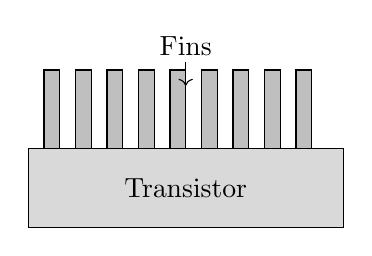
\begin{tikzpicture}
        \draw[fill=gray!30] (0,0) rectangle (4,1);
        \node at (2,0.5) {Transistor};
        \foreach \x in {0.2, 0.6, ..., 3.8} {
            \draw[fill=gray!50] (\x,1) rectangle (\x+0.2,2);
        }
        \node at (2,2.3) {Fins};
        \draw[->] (2,2.1) -- (2,1.8);
    \end{tikzpicture}
    \end{center}

    \begin{itemize}
        \item \textbf{Purpose}: Dissipates excess heat from electronic components (like power transistors) to prevent thermal damage.
        \item \textbf{Types}:
        \begin{itemize}
            \item \textbf{Passive}: Aluminum or copper fins that rely on natural convection.
            \item \textbf{Active}: Uses fans or liquid cooling for forced convection.
        \end{itemize}
        \item \textbf{Thermal Resistance}: Lower thermal resistance ($\theta$, measured in $^\circ$C/W) indicates better heat dissipation capability.
        \item \textbf{Materials}: Copper (best conductivity) or Aluminum (lightweight, cost-effective).
    \end{itemize}

    \mnemonicbox{"HARD sinks - \textbf{H}eat \textbf{A}way using \textbf{R}adiation and \textbf{D}issipation through metal sinks"}
\end{solutionbox}

\questionmarks{1}{c}{7}
\textbf{Describe Thermal Runaway and Thermal Stability. How can overcome thermal run away in transistor?}

\begin{solutionbox}
    \begin{center}
    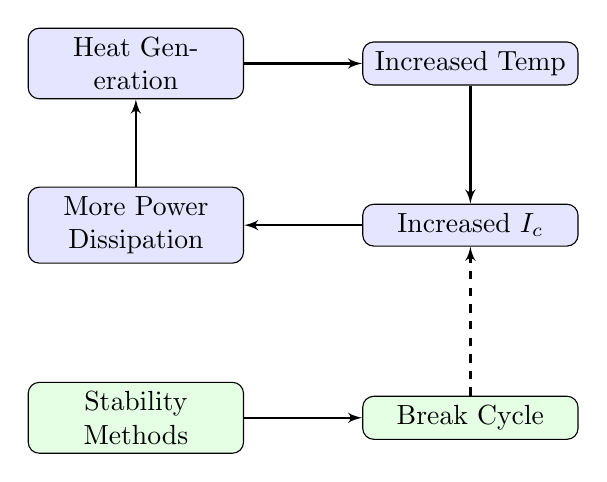
\begin{tikzpicture}[node distance=1.5cm, auto,
        gtu block/.style={rectangle, draw, fill=blue!10, text width=2.5cm, text centered, rounded corners, minimum height=1.5em},
        line/.style={draw, -latex', thick}]
        \node [gtu block] (heat) {Heat Generation};
        \node [gtu block, right=of heat] (temp) {Increased Temp};
        \node [gtu block, below=of temp] (ic) {Increased $I_c$};
        \node [gtu block, left=of ic] (power) {More Power Dissipation};
        
        \path [line] (heat) -- (temp);
        \path [line] (temp) -- (ic);
        \path [line] (ic) -- (power);
        \path [line] (power) -- (heat);
        
        \node [gtu block, below=of power, fill=green!10] (method) {Stability Methods};
        \node [gtu block, right=of method, fill=green!10] (break) {Break Cycle};
        \path [line] (method) -- (break);
        \draw [line, dashed] (break.north) -- (ic.south);
    \end{tikzpicture}
    \end{center}

    \textbf{Thermal Runaway:}
    \begin{itemize}
        \item \textbf{Definition}: A self-accelerating destructive process where the transistor heats up, causing more current to flow, which generates even more heat.
        \item \textbf{chain Reaction}: Increase in temperature $\rightarrow$ Increases leakage current ($I_{CO}$) $\rightarrow$ Increases collector current ($I_C = \beta I_B + (1+\beta)I_{CO}$) $\rightarrow$ Increases Power Dissipation ($P_D = V_{CE} I_C$) $\rightarrow$ Further Temperature Rise.
        \item \textbf{Result}: If unchecked, it leads to the physical destruction of the transistor.
    \end{itemize}

    \textbf{Thermal Stability:}
    \begin{itemize}
        \item \textbf{Definition}: The ability of a circuit to maintain a stable operating point ($Q$-point) despite variations in temperature.
        \item \textbf{Measure}: Quantified by the \keyword{Stability Factor (S)}. Lower values of S indicate better thermal stability.
    \end{itemize}

    \textbf{Overcoming Thermal Runaway:}
    \begin{enumerate}
        \item \textbf{Heat Sinks}: Increasing surface area to dissipate heat into the air.
        \item \textbf{Emitter Resistor}: Using an unbypassed emitter resistor ($R_E$) provides negative feedback. If $I_C$ rises, voltage drop across $R_E$ increases, reducing $V_{BE}$, which reduces $I_B$ and thus opposes the rise in $I_C$.
        \item \textbf{Biasing Methods}: Using circuits like \keyword{Voltage Divider Bias} which offer better stability than fixed bias.
        \item \textbf{Compensation}: Using temperature-sensitive components (thermistors, diodes) in the bias circuit to counteract parameter changes.
    \end{enumerate}

    \mnemonicbox{"SHEER protection - \textbf{S}inks for \textbf{H}eat, \textbf{E}mitter resistors, \textbf{E}xternal cooling, and \textbf{R}obust biasing prevent thermal runaway"}
\end{solutionbox}

\questionmarks{1}{c}{7}
\textbf{Write down types of biasing methods. Explain the voltage divider biasing method in details.}

\begin{solutionbox}
    \textbf{Types of Biasing Methods:}
    \begin{center}
    \begin{tabulary}{\linewidth}{|L|L|L|}
        \hline
        \textbf{Method} & \textbf{Stability} & \textbf{Complexity} \\
        \hline
        Fixed Bias & Poor & Simple \\
        \hline
        Collector Feedback & Medium & Medium \\
        \hline
        Emitter Bias & Good & Medium \\
        \hline
        Voltage Divider & Excellent & Complex \\
        \hline
    \end{tabulary}
    \end{center}

    \textbf{Voltage Divider Biasing:}

    \begin{center}
    \begin{circuitikz}[american]
        \draw (0,0) node[npn](Q){};
        \draw (Q.E) to[R, l=$R_E$] (0,-2) node[ground]{};
        \draw (Q.C) to[R, l=$R_C$] (0,2) -- (0,3) node[vcc]{$+V_{CC}$};
        \draw (Q.C) to[short, -o] (2,0) node[right]{Output};
        \draw (Q.B) -- (-1.5,0);
        \draw (-1.5,0) to[R, l=$R_2$] (-1.5,-2) node[ground]{};
        \draw (-1.5,0) to[R, l=$R_1$] (-1.5,3) node[vcc]{$+V_{CC}$};
        \draw (-1.5,0) to[C, l=$C_{in}$, -o] (-3.5,0) node[left]{Input};
        \draw (2,0) to[C, l=$C_{out}$] (1,0); 
    \end{circuitikz}
    \captionof{figure}{Voltage Divider Bias Circuit}
    \end{center}

    \begin{itemize}
        \item \textbf{Circuit Structure}: Uses two resistors $R_1$ and $R_2$ connected in series across the supply $V_{CC}$ to provide a fixed potential at the base.
        \item \textbf{Operating Principle}: The voltage across $R_2$ (base voltage $V_B$) forward biases the emitter junction.
        \item \textbf{Base Voltage}: $V_B = V_{CC} \times \frac{R_2}{R_1 + R_2}$
        \item \textbf{Stability}: This is the most widely used method because the operating point is almost independent of the transistor's $\beta$.
            \begin{itemize}
                \item If $I_C$ increases due to temperature, $I_E$ increases ($I_E \approx I_C$).
                \item Voltage drop across $R_E$ ($V_E = I_E R_E$) increases.
                \item Since $V_B$ is constant, $V_{BE} = V_B - V_E$ decreases.
                \item Decreased $V_{BE}$ reduces $I_B$, which in turn reduces $I_C$, stabilizing the circuit.
            \end{itemize}
        \item \textbf{Advantage}: High stability factor ($S \approx 1$).
    \end{itemize}

    \mnemonicbox{"DIVE for stability - \textbf{D}ivider \textbf{I}s \textbf{V}ery \textbf{E}ffective for temperature and $\beta$ variations"}
\end{solutionbox}

\questionmarks{2}{a}{3}
\textbf{Explain Stability Factor with features.}

\begin{solutionbox}
    \begin{center}
    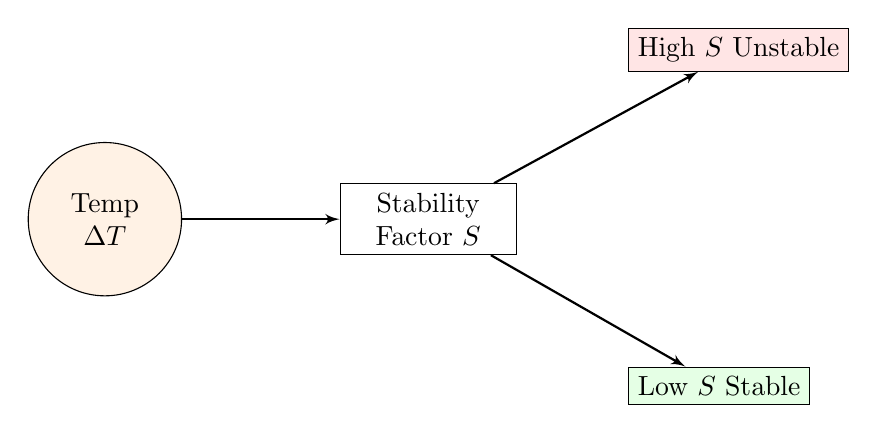
\begin{tikzpicture}[node distance=2cm, auto,
        gtu state/.style={circle, draw, fill=orange!10, text width=1.5cm, text centered, minimum size=1.5cm},
        line/.style={draw, -latex', thick}]
        
        \node [gtu state] (temp) {Temp $\Delta T$};
        \node [rectangle, draw, right=of temp, text width=2cm, align=center] (sf) {Stability Factor $S$};
        \node [rectangle, draw, above right=of sf, fill=red!10] (unstable) {High $S$ Unstable};
        \node [rectangle, draw, below right=of sf, fill=green!10] (stable) {Low $S$ Stable};
        
        \path [line] (temp) -- (sf);
        \path [line] (sf) -- (unstable);
        \path [line] (sf) -- (stable);
    \end{tikzpicture}
    \end{center}

    \begin{itemize}
        \item \textbf{Definition}: Stability factor ($S$) indicates the degree of change in collector current ($I_C$) with respect to the reverse saturation current ($I_{CO}$), keeping $\beta$ and $V_{BE}$ constant.
        \item \textbf{Formula}: $S = \frac{dI_C}{dI_{CO}}$
        \item \textbf{Ideal Value}: Ideally $S=1$. The lower the value of $S$, the better the thermal stability.
        \item \textbf{Significance}: It quantifies how sensitive the Q-point is to temperature variations. A circuit with $S=10$ is less stable than one with $S=2$.
    \end{itemize}

    \mnemonicbox{"LESS is better - \textbf{L}ower values \textbf{E}nsure \textbf{S}table \textbf{S}ystem for temperature changes"}
\end{solutionbox}

\questionmarks{2}{b}{4}
\textbf{Describe direct coupling technique of cascading.}

\begin{solutionbox}
    \begin{center}
    \begin{circuitikz}[american, scale=0.8]
        \draw (0,0) node[npn](Q1){$Q_1$};
        \draw (4,1) node[npn](Q2){$Q_2$};
        
        % Q1 biased
        \draw (Q1.E) to[R, l=$R_{E1}$] (0,-2) node[ground]{};
        \draw (Q1.C) to[R, l=$R_{C1}$] (0,3) node[vcc]{$+V_{CC}$};
        \draw (Q1.B) to[short, -o] (-1,0) node[left]{Input};
        
        % Direct coupling
        \draw (Q1.C) -- (Q2.B);
        
        % Q2 biased
        \draw (Q2.E) to[R, l=$R_{E2}$] (4,-1) node[ground]{};
        \draw (Q2.C) to[R, l=$R_{C2}$] (4,3) node[vcc]{$+V_{CC}$};
        \draw (Q2.C) to[short, -o] (5,1) node[right]{Output};
    \end{circuitikz}
    \end{center}

    \begin{itemize}
        \item \textbf{Definition}: In direct coupling, the output of the first stage is directly connected to the input of the next stage without any coupling capacitor or transformer.
        \item \textbf{Working}: The DC collector voltage of the first stage provides the DC base bias for the second stage.
        \item \textbf{Advantages}:
            \begin{itemize}
                \item Can amplify extremely low frequencies (including DC).
                \item Simple circuit, fewer components (no capacitors/transformers).
                \item Easy to fabricate in Integrated Circuits (ICs).
            \end{itemize}
        \item \textbf{Disadvantages}:
            \begin{itemize}
                \item Thermal drift (shift in Q-point) is amplified stage by stage.
                \item Requires careful design to match DC levels.
            \end{itemize}
    \end{itemize}

    \mnemonicbox{"DIAL for DC - \textbf{D}irect \textbf{I}nterconnection \textbf{A}mplifies \textbf{L}ow frequencies without capacitors"}
\end{solutionbox}

\questionmarks{2}{c}{7}
\textbf{Explain frequency response of two stages RC coupled amplifier.}

\begin{solutionbox}
    \begin{center}
    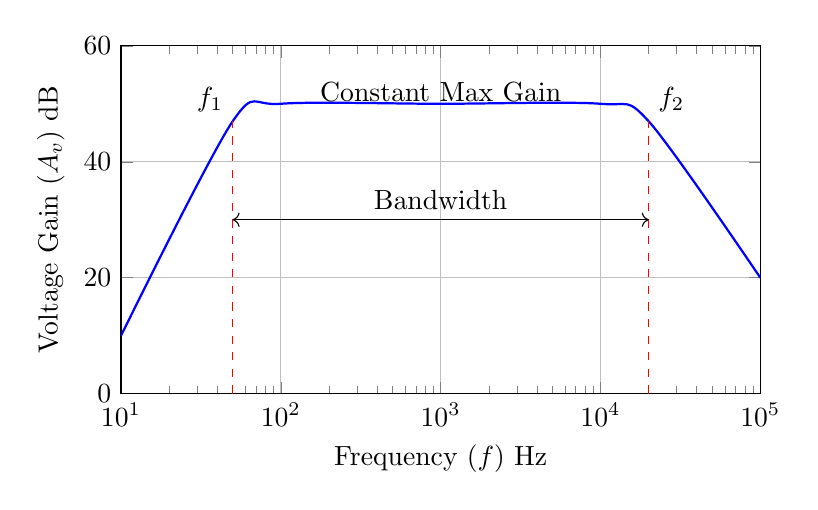
\begin{tikzpicture}
        \begin{semilogxaxis}[
            xlabel={Frequency ($f$) Hz},
            ylabel={Voltage Gain ($A_v$) dB},
            xmin=10, xmax=100000,
            ymin=0, ymax=60,
            width=0.8\linewidth,
            height=6cm,
            grid=major
        ]
        \addplot[thick, smooth, blue] coordinates {
            (10, 10) (50, 47) (100, 50) (1000, 50) (10000, 50) (20000, 47) (100000, 20)
        };
        \draw[dashed, red] (axis cs:50,0) -- (axis cs:50,47) node[above left, black]{$f_1$};
        \draw[dashed, red] (axis cs:20000,0) -- (axis cs:20000,47) node[above right, black]{$f_2$};
        \draw[<->] (axis cs:50, 30) -- (axis cs:20000, 30) node[midway, above]{Bandwidth};
        \node at (axis cs: 1000, 52) {Constant Max Gain};
        \end{semilogxaxis}
    \end{tikzpicture}
    \end{center}

    \textbf{Frequency Response Analysis:}
    \begin{enumerate}
        \item \textbf{Low Frequency Region ($f < f_1$)}:
            \begin{itemize}
                \item The reactance of coupling capacitors ($C_C = 1/2\pi f C$) is high.
                \item A significant voltage drop occurs across $C_C$, reducing the signal reaching the next stage.
                \item The emitter bypass capacitor ($C_E$) also has high reactance, reducing the gain due to negative feedback.
            \end{itemize}
        \item \textbf{Mid Frequency Region ($f_1 < f < f_2$)}:
            \begin{itemize}
                \item Capacitors act as short circuits.
                \item Gain remains constant and maximum.
            \end{itemize}
        \item \textbf{High Frequency Region ($f > f_2$)}:
            \begin{itemize}
                \item Reactance of internal transistor capacitances (inter-electrode capacitance) becomes low.
                \item These shunt the signal to ground, reducing the gain.
                \item Wiring capacitance also contributes to gain reduction.
            \end{itemize}
        \item \textbf{Bandwidth}: The range of frequencies between the lower cut-off ($f_1$) and upper cut-off ($f_2$) where gain is at least 70.7\% (-3dB) of the maximum is the bandwidth.
    \end{enumerate}

    \mnemonicbox{"LMH frequency regions - \textbf{L}ow has rising gain, \textbf{M}iddle has flat gain, \textbf{H}igh has falling gain"}
\end{solutionbox}

\questionmarks{2}{a}{3}
\textbf{Briefly explain bandwidth and gain-bandwidth product of an amplifier.}

\begin{solutionbox}
    \textbf{Bandwidth (BW):}
    \begin{itemize}
        \item It is the range of frequencies over which the amplifier provides satisfactory gain (usually defined as gain being $\ge 70.7\%$ of maximum).
        \item Formula: $BW = f_2 - f_1$, where $f_2$ is upper cut-off and $f_1$ is lower cut-off frequency.
    \end{itemize}

    \textbf{Gain-Bandwidth Product (GBW):}
    \begin{itemize}
        \item For a given amplifier, the product of voltage gain ($A_v$) and bandwidth ($BW$) is a constant.
        \item $GBW = A_v \times BW = \text{Constant}$.
        \item \textbf{Significance}: If we increase gain (e.g., by cascading), the bandwidth decreases, and vice versa. It represents the figure of merit for an amplifier.
    \end{itemize}

    \mnemonicbox{"BIG value - \textbf{B}andwidth and gain \textbf{I}nverse relationship is a \textbf{G}iven constant"}
\end{solutionbox}

\questionmarks{2}{b}{4}
\textbf{Explain effects of emitter bypass capacitor and coupling capacitor on frequency response of an amplifier.}

\begin{solutionbox}
    \begin{center}
    \begin{tabulary}{\linewidth}{|L|L|L|L|}
        \hline
        \textbf{Capacitor} & \textbf{Low Freq} & \textbf{Mid Freq} & \textbf{High Freq} \\
        \hline
        Emitter Bypass ($C_E$) & High reactance, reduces gain (feedback active) & Short circuit, max gain (feedback bypassed) & Short circuit, no effect \\
        \hline
        Coupling ($C_C$) & High reactance, blocks/attenuates signal & Short circuit, allows full signal & Short circuit, no effect \\
        \hline
    \end{tabulary}
    \end{center}

    \begin{itemize}
        \item \textbf{Coupling Capacitor ($C_C$)}:
            \begin{itemize}
                \item Blocks DC to prevent bias interaction between stages.
                \item At low frequencies, its high reactance ($X_C$) causes signal loss, defining the lower cut-off frequency $f_1$.
            \end{itemize}
        \item \textbf{Emitter Bypass Capacitor ($C_E$)}:
            \begin{itemize}
                \item Connected in parallel with $R_E$ to bypass AC signals to ground.
                \item Prevents degeneration (negative feedback) at signal frequencies, thus increasing voltage gain.
                \item At low frequencies, if $X_C$ is high, feedback occurs, reducing gain.
            \end{itemize}
    \end{itemize}

    \mnemonicbox{"CABLE effect - \textbf{C}apacitors \textbf{A}ct as \textbf{B}arriers at \textbf{L}ow frequencies, improving at higher frequencies"}
\end{solutionbox}

\questionmarks{2}{c}{7}
\textbf{Compare transformer coupled amplifier and RC coupled amplifier.}

\begin{solutionbox}
    \begin{center}
    \begin{tabulary}{\linewidth}{|L|L|L|}
        \hline
        \textbf{Parameter} & \textbf{Transformer Coupled} & \textbf{RC Coupled} \\
        \hline
        Coupling Device & Transformer & Capacitor \& Resistor \\
        \hline
        Impedance Matching & Excellent (adjustable via turns ratio) & Poor \\
        \hline
        Frequency Response & Poor (limited due to transformer inductance) & Excellent (wide and flat over audio range) \\
        \hline
        Efficiency & High (no power loss in collector resistor) & Low (power wasted in collector resistor) \\
        \hline
        Size \& Weight & Bulky and Heavy & Compact and Light \\
        \hline
        Cost & Expensive & Inexpensive \\
        \hline
        Application & Power Amplifiers (Impedance matching) & Voltage Amplifiers (Audio/Pre-amps) \\
        \hline
    \end{tabulary}
    \end{center}

    \begin{center}
    \begin{minipage}{0.45\linewidth}
        \centering
        \textbf{Transformer Coupled}
        \begin{circuitikz}[american, scale=0.6]
             \draw (0,0) node[npn](Q){};
             \draw (Q.E) node[ground]{};
             \draw (Q.C) to[L] (0,2); % Primary
             \draw (0.5,2) to[L] (0.5,0); % Secondary
             \draw (0.25, 0) -- (0.25, 2); % Core
             \draw (0,2) -- (0,2.5) node[vcc]{};
        \end{circuitikz}
    \end{minipage}
    \begin{minipage}{0.45\linewidth}
        \centering
        \textbf{RC Coupled}
        \begin{circuitikz}[american, scale=0.6]
             \draw (0,0) node[npn](Q){};
             \draw (Q.E) node[ground]{};
             \draw (Q.C) to[R] (0,2.5) node[vcc]{};
             \draw (Q.C) to[C] (2,1);
        \end{circuitikz}
    \end{minipage}
    \end{center}

    \mnemonicbox{"TREE factors - \textbf{TR}ansformers provide \textbf{E}fficiency and \textbf{E}xcellent impedance matching, RC provides Cost savings"}
\end{solutionbox}

\questionmarks{3}{a}{3}
\textbf{Describe the transistorized tuned amplifier.}

\begin{solutionbox}
    \begin{center}
    \begin{circuitikz}[american]
        \draw (0,0) node[npn](Q){};
        \draw (Q.E) node[ground]{};
        \draw (Q.C) -- (0,1.5);
        % Tank Circuit
        \draw (-1,1.5) -- (1,1.5);
        \draw (-1,1.5) to[L, l=$L$] (-1,3.5);
        \draw (1,1.5) to[C, l=$C$] (1,3.5);
        \draw (-1,3.5) -- (1,3.5);
        \draw (0,3.5) -- (0,4) node[vcc]{$+V_{CC}$};
        
        \draw (Q.B) to[short, -o] (-2,0) node[left]{Input};
        \draw (Q.C) to[C, -o] (2,0) node[right]{Output};
        
        % Biasing resistors (simplified)
        \draw (-1.5,0) to[R, l=$R_B$] (-1.5,3) node[vcc]{};
    \end{circuitikz}
    \end{center}

    \begin{itemize}
        \item \textbf{Definition}: An amplifier that uses a parallel LC circuit (tank circuit) as the collector load to amplify a specific narrow band of frequencies.
        \item \textbf{Resonance}: The LC circuit resonates at frequency $f_r = \frac{1}{2\pi\sqrt{LC}}$.
        \item \textbf{Gain}: At resonance, the impedance of the tank circuit is maximum (resistive), resulting in maximum voltage gain.
        \item \textbf{Applications}: Used in the Radio Frequency (RF) and Intermediate Frequency (IF) stages of receivers.
    \end{itemize}

    \mnemonicbox{"TRIP to resonance - \textbf{T}uned \textbf{R}esonant circuits \textbf{I}mprove \textbf{P}erformance at specific frequencies"}
\end{solutionbox}

\questionmarks{3}{b}{4}
\textbf{Explain in brief Direct coupled amplifier.}

\begin{solutionbox}
    \begin{center}
    \begin{circuitikz}[american, scale=0.8]
        \draw (0,0) node[npn](Q1){$Q_1$};
        \draw (3,1) node[npn](Q2){$Q_2$};
        \draw (Q1.C) -- (Q2.B); % Direct coupling
        \draw (Q1.E) node[ground]{};
        \draw (Q2.E) to[R] (3,-1) node[ground]{};
        \draw (Q1.C) to[R] (0,3) node[vcc]{$+V_{CC}$};
        \draw (Q2.C) to[R] (3,3) node[vcc]{};
        \draw (Q2.C) to[short, -o] (4,1) node[right]{Output};
    \end{circuitikz}
    \end{center}

    \begin{itemize}
        \item \textbf{Definition}: A multi-stage amplifier where the output of one stage is connected directly to the input of the next stage without any reactive components.
        \item \textbf{Characteristics}:
            \begin{itemize}
                \item \textbf{Low Frequency Response}: Excellent, can amplify down to DC (0 Hz).
                \item \textbf{Simplicity}: Requires fewer components (no bulky capacitors).
                \item \textbf{Issues}: Suffers from \keyword{DC drift} (thermal instability shifting the operating point).
            \end{itemize}
        \item \textbf{Application}: Linear ICs, Operational Amplifiers, low-frequency instrumentation.
    \end{itemize}
    \mnemonicbox{"COLD advantages - \textbf{C}ompact design, \textbf{O}utstanding low-frequency response, \textbf{L}ess components, \textbf{D}irect connection"}
\end{solutionbox}

\questionmarks{3}{c}{7}
\textbf{Describe the importance of h parameters in two port network. Draw h-parameters circuit for CE amplifier.}

\begin{solutionbox}
    \textbf{Transistor h-parameter Model (CE Configuration):}
    \begin{center}
    \begin{circuitikz}[american, scale=0.9]
        % Input loop
        \draw (0,0) to[short, o-] (1,0) to[R, l=$h_{ie}$] (3,0) to[cV, l=$h_{re}V_{ce}$] (5,0) to[short, -o] (5,-2);
        \draw (0,-2) to[short, o-o] (5,-2);
        \node at (0, -1) {$V_{in}$};
        \node at (2.5, -2.5) {Emitter (E)};
        \node at (0, 0.5) {Base (B)};
        
        % Output loop
        \draw (7,0) to[cI, l=$h_{fe}I_b$] (7,-2); % Current source downward
        \draw (7,0) -- (9,0) to[R, l=$\frac{1}{h_{oe}}$] (9,-2) -- (7,-2);
        \draw (9,0) to[short, -o] (11,0); 
        \draw (9,-2) to[short, -o] (11,-2);
        \node at (11, -1) {$V_{ce}$};
        \node at (11, 0.5) {Collector (C)};
        \draw (5,-2) -- (7,-2); % Common ground line
    \end{circuitikz}
    \captionof{figure}{h-parameter Equivalent Circuit for CE}
    \end{center}

    \textbf{Importance of h-parameters:}
    \begin{itemize}
        \item \textbf{Hybrid Nature}: They use a mix of units ($\Omega$, Siemens, dimensionless), hence "hybrid".
        \item \textbf{Ease of Measurement}: They are defined based on open-circuit and short-circuit conditions which are easy to implement practically.
        \item \textbf{Accuracy}: They provide accurate results for small-signal analysis at low frequencies.
        \item \textbf{Standardization}: Manufacturers specify transistor characteristics using these parameters ($h_{fe}$, $h_{ie}$, etc.).
    \end{itemize}

    \textbf{CE Parameters:}
    \begin{itemize}
        \item $h_{ie}$ ($h_{11}$): Input Impedance.
        \item $h_{re}$ ($h_{12}$): Reverse Voltage Ratio.
        \item $h_{fe}$ ($h_{21}$): Forward Current Gain.
        \item $h_{oe}$ ($h_{22}$): Output Admittance.
    \end{itemize}

    \mnemonicbox{"FINE parameters - \textbf{F}our \textbf{I}nterconnected \textbf{N}etwork \textbf{E}lements define transistor completely"}
\end{solutionbox}

\questionmarks{3}{a}{3}
\textbf{Compare transformer coupled amplifier and direct coupled amplifier.}

\begin{solutionbox}
    \begin{center}
    \begin{tabulary}{\linewidth}{|L|L|L|}
        \hline
        \textbf{Parameter} & \textbf{Transformer Coupled} & \textbf{Direct Coupled} \\
        \hline
        DC Isolation & Complete & None \\
        \hline
        Freq Response & Poor (limited band) & Excellent (down to DC) \\
        \hline
        Size/Weight & Bulky/Heavy & Compact/Light \\
        \hline
        Impedance Matching & Excellent & Poor \\
        \hline
        Cost & High & Low \\
        \hline
        Drift & No drift problem & Severe drift problem \\
        \hline
    \end{tabulary}
    \end{center}
    \mnemonicbox{"TIP for selection - \textbf{T}ransformer for \textbf{I}mpedance matching and \textbf{P}ower transfer, Direct for low frequencies"}
\end{solutionbox}

\questionmarks{3}{b}{4}
\textbf{Draw and Explain circuit diagram of common emitter amplifier.}

\begin{solutionbox}
    \begin{center}
    \begin{circuitikz}[american]
        \draw (0,0) node[npn](Q){};
        \draw (Q.E) to[R, l=$R_E$] (0,-2) node[ground]{};
        % Bypass Cap
        \draw (0,-0.5) -- (1.5,-0.5) to[C, l=$C_E$] (1.5,-2) -- (0,-2);
        
        \draw (Q.C) to[R, l=$R_C$] (0,2) -- (0,3) node[vcc]{$+V_{CC}$};
        \draw (Q.C) to[C, l=$C_{out}$, -o] (2,0) node[right]{Output};
        
        % Voltage Divider Check
        \draw (Q.B) -- (-1.5,0);
        \draw (-1.5,0) to[R, l=$R_2$] (-1.5,-2) node[ground]{};
        \draw (-1.5,0) to[R, l=$R_1$] (-1.5,3) node[vcc]{};
        
        \draw (-1.5,0) to[C, l=$C_{in}$, -o] (-3.5,0) node[left]{Input};
    \end{circuitikz}
    \end{center}

    \begin{itemize}
        \item \textbf{Circuit}: Uses Voltage Divider Bias ($R_1, R_2$) for stability. Capacitors $C_{in}$ and $C_{out}$ block DC. $C_E$ bypasses $R_E$ to prevent AC gain application.
        \item \textbf{Operation}: Small AC input at base varies base current, which is amplified by $\beta$ at the collector.
        \item \textbf{Phase Shift}: Output is \keyword{180$^{\circ}$ out of phase} with input.
        \item \textbf{Characteristics}: Moderate input/output impedance, high voltage and current gain.
    \end{itemize}
    \mnemonicbox{"GAIN characteristics - \textbf{G}ood \textbf{A}mplification with \textbf{I}nverted output and \textbf{N}otable efficiency"}
\end{solutionbox}

\questionmarks{3}{c}{7}
\textbf{Draw Transistor Two Port Network and describe h-parameters for it. Write down advantages of hybrid parameters.}

\begin{solutionbox}
    \textbf{Two-Port Network:}
    \begin{center}
    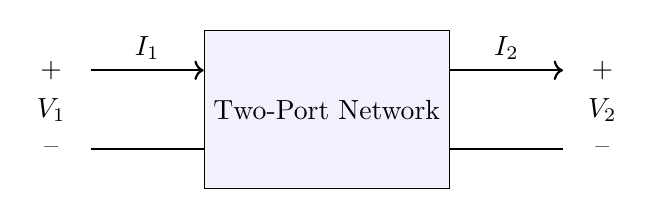
\begin{tikzpicture}[
        box/.style={draw, rectangle, minimum width=3cm, minimum height=2cm, fill=blue!5},
        arrow/.style={->, thick}
    ]
        \node (net) [box] {Two-Port Network};
        
        % Input Port
        \draw [arrow] (-3, 0.5) -- node[above] {$I_1$} (net.west |- 0, 0.5);
        \node at (-3.5, 0.5) {+};
        \node at (-3.5, -0.5) {--};
        \node at (-3.5, 0) {$V_1$};
        \draw (-3, -0.5) -- (net.west |- 0, -0.5);
        
        % Output Port
        \draw [arrow] (net.east |- 0, 0.5) -- node[above] {$I_2$} (3, 0.5);
        \node at (3.5, 0.5) {+};
        \node at (3.5, -0.5) {--};
        \node at (3.5, 0) {$V_2$};
        \draw (net.east |- 0, -0.5) -- (3, -0.5);
    \end{tikzpicture}
    \end{center}

    \textbf{h-Parameter Equations:}
    \[ V_1 = h_{11}I_1 + h_{12}V_2 \]
    \[ I_2 = h_{21}I_1 + h_{22}V_2 \]

    \textbf{Advantages:}
    \begin{itemize}
        \item \textbf{Realizable}: Parameters correspond to easy-to-measure physical quantities (impedance, gain, etc.).
        \item \textbf{Low Frequency Suitability}: Highly accurate for analyzing audio frequency circuits.
        \item \textbf{Universal}: Apply to any active device (BJT, FET) treated as a black box.
        \item \textbf{Dimensional Variety}: Since they mix ohms, siemens, and dimensionless ratios, they flexibly describe complex interactions.
    \end{itemize}
    \mnemonicbox{"SMART parameters - \textbf{S}imple \textbf{M}easurement, \textbf{A}ccurate modeling, \textbf{R}eliable, \textbf{T}emperature-stable"}
\end{solutionbox}

\questionmarks{4}{a}{3}
\textbf{Explain Darlington pair and its applications.}

\begin{solutionbox}
    \begin{center}
    \begin{circuitikz}[american]
        \draw (0,0) node[npn](Q1){$Q_1$};
        \draw (2,-0.5) node[npn](Q2){$Q_2$};
        
        \draw (Q1.C) -- (Q2.C); % Collectors connected
        \draw (Q1.C) -- (1,2) node[above]{$C$};
        
        \draw (Q1.E) -- (Q2.B); % Emitter to Base
        
        \draw (Q1.B) -- (-1,0) node[left]{$B$};
        \draw (Q2.E) -- (2,-1.5) node[below]{$E$};
    \end{circuitikz}
    \end{center}

    \begin{itemize}
        \item \textbf{Definition}: Two transistors connected such that the emitter current of the first becomes the base current of the second, often packaged as a single device.
        \item \textbf{Current Gain}: The total current gain is the product of individual gains ($\beta_{total} \approx \beta_1 \times \beta_2$). Extremely high.
        \item \textbf{Input Impedance}: Very high.
        \item \textbf{Applications}: High current drivers (relays, motors), input stages of high-impedance amplifiers.
    \end{itemize}
    \mnemonicbox{"HIGH gain - \textbf{H}ugely \textbf{I}ncreased \textbf{G}ain from \textbf{H}arnessing two transistors"}
\end{solutionbox}

\questionmarks{4}{b}{4}
\textbf{Describe the diode clamper circuit with necessary diagram.}

\begin{solutionbox}
    \textbf{Positive Clamper:}
    \begin{center}
    \begin{circuitikz}[american]
        \draw (0,0) node[left]{Input} to[C, l=$C$] (2,0) -- (4,0) node[right]{Output};
        \draw (3,0) to[R, l=$R$] (3,-2) node[ground]{};
        \draw (2,-2) node[ground]{} to[D*, l=$D$] (2,0); % Points Up
    \end{circuitikz}
    \end{center}

    \begin{itemize}
        \item \textbf{Function}: Adds a DC shift to the input signal without changing its shape (DC Restorer).
        \item \textbf{Positive Clamper}: Shifts the signal UP so negative peaks sit on zero (or reference) level.
        \item \textbf{Operation}:
            \begin{itemize}
                \item During the negative half-cycle, Diode conducts, charging Capacitor to $V_p$ (polarity: + on right).
                \item During the positive half-cycle, Diode is reverse biased.
                \item Output voltage $V_o = V_{in} + V_C = V_{in} + V_p$.
            \end{itemize}
    \end{itemize}
    \mnemonicbox{"CAPS effect - \textbf{C}apacitor \textbf{A}nd diode \textbf{P}air \textbf{S}hifts signal by exact DC level"}
\end{solutionbox}

\questionmarks{4}{c}{7}
\textbf{Explain the construction, working and applications of OLED.}

\begin{solutionbox}
    \textbf{OLED Construction:}
    \begin{center}
    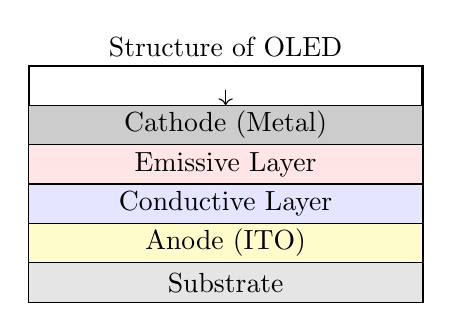
\begin{tikzpicture}
        \draw[thick] (0,0) rectangle (5,3);
        
        \draw[fill=gray!20] (0,0) rectangle (5,0.5); \node at (2.5, 0.25) {Substrate};
        \draw[fill=yellow!20] (0,0.5) rectangle (5,1.0); \node at (2.5, 0.75) {Anode (ITO)};
        \draw[fill=blue!10] (0,1.0) rectangle (5,1.5); \node at (2.5, 1.25) {Conductive Layer};
        \draw[fill=red!10] (0,1.5) rectangle (5,2.0); \node at (2.5, 1.75) {Emissive Layer};
        \draw[fill=gray!40] (0,2.0) rectangle (5,2.5); \node at (2.5, 2.25) {Cathode (Metal)};
        
        \node[above] at (2.5,3) {Structure of OLED};
        \draw[->] (2.5, 2.7) -- (2.5, 2.5);
    \end{tikzpicture}
    \end{center}

    \begin{itemize}
        \item \textbf{Construction}: Consists of organic semiconductor layers sandwiched between two electrodes (Anode and Cathode) deposited on a substrate.
        \item \textbf{Layers}:
            \begin{itemize}
                \item \textbf{Emissive Layer}: Organic molecules that emit light.
                \item \textbf{Conductive Layer}: Transports holes from anode.
            \end{itemize}
        \item \textbf{Working}:
            \begin{itemize}
                \item When voltage is applied, current flows from cathode to anode.
                \item Cathode gives electrons to emissive layer; Anode removes electrons (adds holes) to conductive layer.
                \item Electrons and holes recombine in the emissive layer, releasing energy as photons (Light).
            \end{itemize}
        \item \textbf{Applications}: Premium smartphones, TVs, flexible displays, digital signage.
    \end{itemize}
    \mnemonicbox{"OLED benefits - \textbf{O}rganic materials, \textbf{L}ightweight design, \textbf{E}fficient operation, \textbf{D}irect emission"}
\end{solutionbox}

\questionmarks{4}{a}{3}
\textbf{Explain Short note on LDR.}

\begin{solutionbox}
    \begin{center}
    \begin{tikzpicture}
        % Symbol
        \draw[thick] (0,0) rectangle (1,2);
        \draw (0.5,0) -- (0.5,-0.5);
        \draw (0.5,2) -- (0.5,2.5);
        \draw[->, thick, zigzag] (-0.5, 1.5) -- (0.2, 1);
        \draw[->, thick, zigzag] (-0.5, 1) -- (0.2, 0.5);
        \node[below] at (0.5, -0.5) {Symbol};
        
        % Structure
        \draw[thick] (3,0) circle (1);
        \draw[decorate, decoration={snake}] (2.5,0) -- (3.5,0); % Zigzag track
        \node[below] at (3, -1.2) {Structure (Top View)};
    \end{tikzpicture}
    \end{center}

    \begin{itemize}
        \item \textbf{Full Form}: Light Dependent Resistor.
        \item \textbf{Principle}: Photoconductivity. Resistance decreases when light intensity increases.
        \item \textbf{Material}: Made of Cadmium Sulfide (CdS).
        \item \textbf{Operation}: In dark, resistance is very high (M$\Omega$). In light, electron-hole pairs are generated, resistance drops (to few 100 $\Omega$).
        \item \textbf{Use}: Automatic street lights, camera exposure meters.
    \end{itemize}
    \mnemonicbox{"DARK increases resistance - \textbf{D}ecreasing light \textbf{A}nd \textbf{R}ising darkness \textbf{K}eep resistance high"}
\end{solutionbox}

\questionmarks{4}{b}{4}
\textbf{Describe the diode clipper circuit with necessary diagram.}

\begin{solutionbox}
    \textbf{Positive Clipper (Series):}
    \begin{center}
    \begin{circuitikz}[american]
        \draw (0,0) node[left]{Input} to[D, l=$D$, invert] (2,0) -- (4,0) node[right]{Output};
        \draw (3,0) to[R, l=$R_L$] (3,-2) node[ground]{};
        \draw (0,0) to[open, v=$V_{in}$] (0,-2);
        \draw (0,-2) node[ground]{};
    \end{circuitikz}
    \end{center}

    \begin{itemize}
        \item \textbf{Definition}: A circuit that removes (clips) a portion of the input signal waveform.
        \item \textbf{Positive Clipper}: Removes the positive half cycle.
        \item \textbf{Working}:
            \begin{itemize}
                \item During positive half cycle, Diode is reverse biased (Open). No current flows to load. Output = 0.
                \item During negative half cycle, Diode is forward biased (Short). Current flows. Output = Input (approx).
            \end{itemize}
        \item \textbf{Applications}: Waveform shaping, protection against voltage spikes.
    \end{itemize}
    \mnemonicbox{"CLIP waves - \textbf{C}ircuit \textbf{L}imits \textbf{I}nput \textbf{P}eaks by using diode conduction"}
\end{solutionbox}

\questionmarks{4}{c}{7}
\textbf{Explain Half Wave and Full wave Voltage Doubler.}

\begin{solutionbox}
    \textbf{Half-Wave Voltage Doubler:}
    \begin{center}
    \begin{circuitikz}[american, scale=0.8]
        \draw (0,0) node[left]{AC} to[C, l=$C_1$] (2,0);
        \draw (2,0) to[D, l=$D_1$, invert] (2,-2) node[ground]{}; % D1 conducts on -ve cycle to charge C1
        \draw (2,0) to[D, l=$D_2$] (4,0) -- (5,0) node[right]{Output};
        \draw (4,0) to[C, l=$C_2$] (4,-2) node[ground]{};
        \draw (0,-2) node[ground]{};
    \end{circuitikz}
    \end{center}

    \begin{itemize}
        \item \textbf{Operation}:
            \begin{itemize}
                \item Negative Cycle: $D_1$ conducts, $C_1$ charges to $V_m$ (peak).
                \item Positive Cycle: $D_2$ conducts. Input voltage ($V_m$) + $C_1$ voltage ($V_m$) charges $C_2$ to $2V_m$.
            \end{itemize}
        \item \textbf{Output}: DC voltage $\approx 2V_m$.
    \end{itemize}

    \textbf{Full-Wave Voltage Doubler:}
    \begin{center}
    \begin{circuitikz}[american, scale=0.8]
        \draw (0,0) node[left]{AC} -- (2,0);
        \draw (2,0) to[D, l=$D_1$] (4,0); % Top branch
        \draw (2,0) to[D, l=$D_2$, invert] (4,-2); % Bottom branch
        \draw (4,0) to[C, l=$C_1$] (4,-1) -- (2,-1) to[short] (0,-1) node[left]{AC Ret};
        \draw (4,-1) to[C, l=$C_2$] (4,-2);
        \draw (4,0) -- (6,0) node[right]{+ Output};
        \draw (4,-2) -- (6,-2) node[right]{- Output};
    \end{circuitikz}
    \end{center}

    \begin{itemize}
        \item \textbf{Operation}: Charges one capacitor during the positive cycle and the other during the negative cycle. The output is the sum across both.
        \item \textbf{Advantage}: Higher ripple frequency (easier to filter).
    \end{itemize}
    \mnemonicbox{"CHASE 2V - \textbf{C}apacitors \textbf{H}old \textbf{A}lternating \textbf{S}upply \textbf{E}nergy to produce 2$\times$ Voltage"}
\end{solutionbox}

\questionmarks{5}{a}{3}
\textbf{Draw circuit diagram for +5v Power Supply using its IC and explain in brief.}

\begin{solutionbox}
    \begin{center}
    \begin{circuitikz}[american, scale=0.8]
        % Transformer
        \draw (0,0) node[transformer core](T){};
        \node[left] at (T.A1) {AC In};
        
        \draw (T.B1) to[short] (2,1) to[D] (3,2); % Top Left D
        \draw (2,1) to[D, invert] (3,0); % Bot Left D
        \draw (T.B2) to[short] (4,1) to[D] (3,2); % Top Right D
        \draw (4,1) to[D, invert] (3,0); % Bot Right D (Invert means cathode at start?)
        % Standard bridge:
        % 4 diodes.
        % Node Top (3,2) is +DC. Node Bot (3,0) is -DC (GND).
        % AC inputs at (2,1) and (4,1).
        
        % Filter Cap
        \draw (3,2) -- (5,2) to[C, l=$C_1$] (5,0) -- (3,0);
        
        % Regulator 7805
        \draw (6,2) node[draw, rectangle, minimum width=1.5cm, minimum height=1cm, anchor=west] (IC) {7805};
        \draw (5,2) -- (IC.west);
        \draw (5,0) -- (6,0) -- (IC.south); % GND pin
        \draw (IC.east) -- (9,2) node[right]{+5V};
        
        % Output Cap
        \draw (8.5,2) to[C, l=$C_2$] (8.5,0);
        \draw (6,0) -- (9,0) node[right]{GND};
    \end{circuitikz}
    \end{center}

    \begin{itemize}
        \item \textbf{Components}:
            \begin{itemize}
                \item \textbf{Transformer}: Steps down AC mains (230V to 9V).
                \item \textbf{Rectifier}: Converts AC to pulsating DC.
                \item \textbf{Filter ($C_1$)}: Smooths pulsations to produce unregulated DC.
                \item \textbf{IC 7805}: Voltage regulator that provides constant +5V output.
                \item \textbf{Capacitor ($C_2$)}: Removes high-frequency noise/transients.
            \end{itemize}
        \item \textbf{Working}: The AC is rectified, filtered, and then regulated by the 7805 IC which dissipates excess voltage as heat to maintain 5V.
    \end{itemize}
    \mnemonicbox{"FIRM voltage - \textbf{F}iltered \textbf{I}nput, \textbf{R}egulated by 7805 \textbf{M}akes stable voltage"}
\end{solutionbox}

\questionmarks{5}{b}{4}
\textbf{Discuss load regulation and line regulation in reference to power supply.}

\begin{solutionbox}
    \begin{center}
    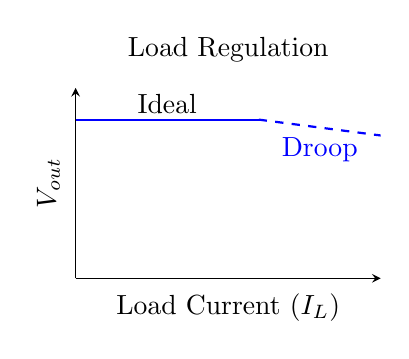
\begin{tikzpicture}
        \begin{axis}[
            width=0.45\linewidth, height=4cm,
            xlabel={Load Current ($I_L$)}, ylabel={$V_{out}$},
            title={Load Regulation},
            ymin=0, ymax=6, xmin=0, xmax=10,
            xtick=\empty, ytick=\empty,
            axis lines=left
        ]
        \draw[thick, blue] (axis cs:0,5) -- (axis cs:6,5);
        \draw[thick, blue, dashed] (axis cs:6,5) -- (axis cs:10,4.5) node[midway, below]{Droop};
        \node at (axis cs:3,5.5) {Ideal};
        \end{axis}
    \end{tikzpicture}
    \hspace{0.5cm}
    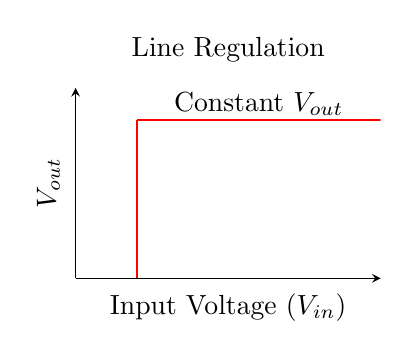
\begin{tikzpicture}
        \begin{axis}[
            width=0.45\linewidth, height=4cm,
            xlabel={Input Voltage ($V_{in}$)}, ylabel={$V_{out}$},
            title={Line Regulation},
            ymin=0, ymax=6, xmin=0, xmax=10,
            xtick=\empty, ytick=\empty,
            axis lines=left
        ]
        \draw[thick, red] (axis cs:2,0) -- (axis cs:2,5);
        \draw[thick, red] (axis cs:2,5) -- (axis cs:10,5);
        \node at (axis cs:6,5.5) {Constant $V_{out}$};
        \end{axis}
    \end{tikzpicture}
    \end{center}

    \begin{itemize}
        \item \textbf{Load Regulation}:
            \begin{itemize}
                \item \textbf{Definition}: The ability of a power supply to maintain constant output voltage despite changes in load current.
                \item \textbf{Formula}: $\%LR = \frac{V_{NoLow} - V_{FullLoad}}{V_{FullLoad}} \times 100$
                \item \textbf{Ideal}: 0\% (Perfectly stiff voltage source).
            \end{itemize}
        \item \textbf{Line Regulation}:
            \begin{itemize}
                \item \textbf{Definition}: The ability to maintain constant output voltage despite changes in AC input (mains) voltage.
                \item \textbf{Formula}: $\%SR = \frac{\Delta V_{out}}{\Delta V_{in}} \times 100$
                \item \textbf{Significance}: Ensures voltage stability during brownouts or surges.
            \end{itemize}
    \end{itemize}
    \mnemonicbox{"LIVER health - \textbf{LI}ne regulation for \textbf{V}ariations in Input, load regulation for \textbf{E}xternal \textbf{R}esistance changes"}
\end{solutionbox}

\questionmarks{5}{c}{7}
\textbf{Explain adjustable voltage regulator using LM317 with circuit diagram.}

\begin{solutionbox}
    \begin{center}
    \begin{circuitikz}[american]
        \draw (0,0) node[draw, rectangle, minimum width=2cm, minimum height=1cm] (IC) {LM317};
        \node at (IC.west) [left] {In};
        \node at (IC.east) [right] {Out};
        \node at (IC.south) [below] {Adj};
        
        \draw (-2,0) to[short, o-] (IC.west);
        \node at (-2,0) [left] {$V_{in}$};
        
        \draw (IC.east) -- (2,0) to[short, -o] (4,0) node[right]{$V_{out}$};
        
        % Resistors
        \draw (2,0) to[R, l=$R_1$] (2,-2);
        \draw (IC.south) -- (0,-2) -- (2,-2) -- (2,-3);
        \draw (2,-3) to[vR, l=$R_2$] (2,-5) node[ground]{};
        
        \draw (4,0) to[C, l=$C_{out}$] (4,-2) -- (4,-5) node[ground]{};
        \draw (-1,0) to[C, l=$C_{in}$] (-1,-2) -- (-1,-5) node[ground]{};
    \end{circuitikz}
    \end{center}

    \begin{itemize}
        \item \textbf{Description}: LM317 is a popular adjustable positive voltage regulator capable of supplying more than 1.5A over a 1.25V to 37V output range.
        \item \textbf{Working}:
            \begin{itemize}
                \item It develops a nominal 1.25V reference voltage ($V_{ref}$) between the Output and Adjustment terminal.
                \item This reference voltage is impressed across resistor $R_1$, causing a constant current $I_1$ to flow.
                \item This current also flows through $R_2$ (ignoring small $I_{Adj}$).
            \end{itemize}
        \item \textbf{formula}: $V_{out} = 1.25V \left( 1 + \frac{R_2}{R_1} \right) + I_{Adj}R_2$
        \item \textbf{Applications}: Variable bench power supplies, battery chargers.
    \end{itemize}
    \mnemonicbox{"VAIR control - \textbf{V}ariable \textbf{A}djustable \textbf{I}ntegrated \textbf{R}egulator controls voltage precisely"}
\end{solutionbox}

\questionmarks{5}{a}{3}
\textbf{Explain working of solar battery charger circuits.}

\begin{solutionbox}
    \begin{center}
    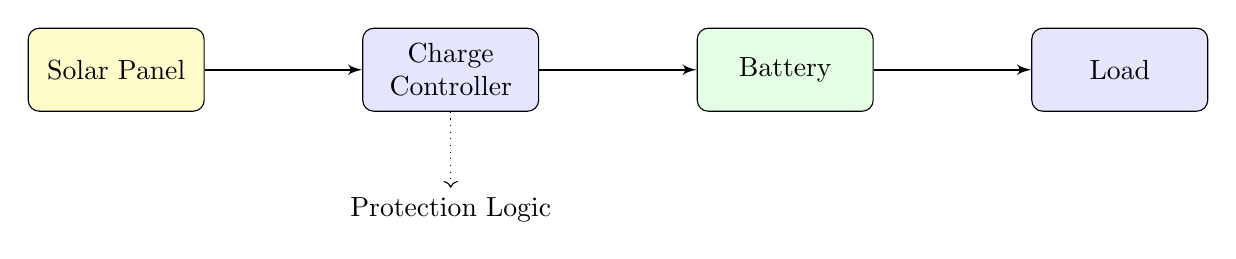
\begin{tikzpicture}[node distance=2cm, auto,
        block/.style={rectangle, draw, fill=blue!10, text width=2cm, text centered, rounded corners, minimum height=3em},
        line/.style={draw, -latex', thick}]
        \node [block, fill=yellow!20] (solar) {Solar Panel};
        \node [block, right=of solar] (ctrl) {Charge Controller};
        \node [block, right=of ctrl, fill=green!10] (batt) {Battery};
        \node [block, right=of batt] (load) {Load};
        
        \path [line] (solar) -- (ctrl);
        \path [line] (ctrl) -- (batt);
        \path [line] (batt) -- (load);
        
        \draw[->, dotted] (ctrl) -- ++(0,-1.5) node[below] {Protection Logic};
    \end{tikzpicture}
    \end{center}

    \begin{itemize}
        \item \textbf{Function}: Converts solar energy into electrical energy to charge a rechargeable battery.
        \item \textbf{Charge Controller}:
            \begin{itemize}
                \item Regulates voltage and current from solar panels.
                \item Prevents \keyword{Overcharging} (which damages battery) and \keyword{Reverse Current} (battery discharging into panel at night).
            \end{itemize}
        \item \textbf{Operation}: Panel generates DC $\rightarrow$ Controller adjusts levels $\rightarrow$ Battery stores energy $\rightarrow$ Load uses it.
    \end{itemize}
    \mnemonicbox{"SCBL system - \textbf{S}olar panel \textbf{C}onverts sunlight, \textbf{B}attery stores, \textbf{L}oad consumes"}
\end{solutionbox}

\questionmarks{5}{b}{4}
\textbf{Explain working of UPS.}

\begin{solutionbox}
    \begin{center}
    \begin{tikzpicture}[node distance=2.5cm, auto,
        block/.style={rectangle, draw, text width=2cm, text centered, minimum height=2em},
        line/.style={draw, -latex', thick}]
        
        \node (ac) {AC Mains};
        \node [block, right=of ac] (rect) {Rectifier / Charger};
        \node [block, right=of rect] (batt) {Battery};
        \node [block, right=of batt] (inv) {Inverter};
        \node [right=of inv] (load) {AC Output};
        
        \node [block, above=of batt, text width=4cm] (switch) {Transfer Switch / Bypass};
        
        \path [line] (ac) -- (rect);
        \path [line] (rect) -- (batt);
        \path [line] (batt) -- (inv);
        \path [line] (inv) -- (load);
        
        \draw [line, dashed] (ac) |- (switch);
        \draw [line, dashed] (switch) -| (load);
        
    \end{tikzpicture}
    \end{center}

    \begin{itemize}
        \item \textbf{Full Form}: Uninterruptible Power Supply.
        \item \textbf{Normal Mode}: AC mains powers the load (directly or via rectification) and charges the battery.
        \item \textbf{Backup Mode}: When mains fail, the Inverter converts DC from the Battery back to AC to power the load.
        \item \textbf{Transfer Switch}: Seamlessly switches between Mains and Inverter output to assume zero downtime.
    \end{itemize}
    \mnemonicbox{"PRIME power - \textbf{P}ower \textbf{R}emains \textbf{I}ntact during \textbf{M}ains \textbf{E}lectricity problems"}
\end{solutionbox}

\questionmarks{5}{c}{7}
\textbf{Draw and explain SMPS block diagram with its advantages and disadvantages.}

\begin{solutionbox}
    \begin{center}
    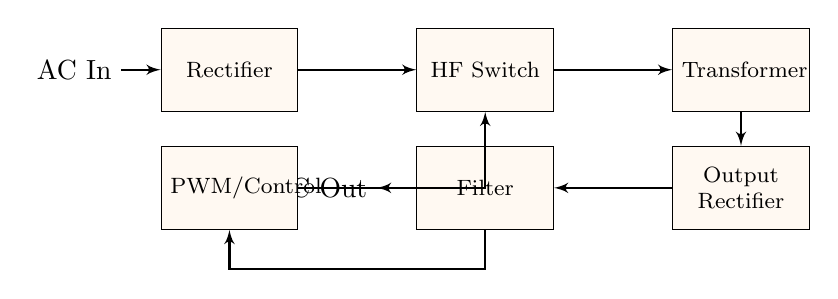
\begin{tikzpicture}[node distance=1.5cm, auto,
        block/.style={rectangle, draw, fill=orange!5, text width=1.5cm, text centered, font=\footnotesize, minimum height=3em},
        line/.style={draw, -latex', thick}]
        
        \node (in) {AC In};
        \node [block, right=0.5cm of in] (rect1) {Rectifier};
        \node [block, right=of rect1] (switch) {HF Switch};
        \node [block, right=of switch] (trans) {Transformer};
        \node [block, below of=trans] (rect2) {Output Rectifier};
        \node [block, left=of rect2] (filter) {Filter};
        \node [left=0.5cm of filter] (out) {DC Out};
        
        \node [block, left=of filter] (ctrl) {PWM/Control};
        
        \path [line] (in) -- (rect1);
        \path [line] (rect1) -- (switch);
        \path [line] (switch) -- (trans);
        \path [line] (trans) -- (rect2);
        \path [line] (rect2) -- (filter);
        \path [line] (filter) -- (out);
        
        \draw [line] (filter.south) |- ++(0,-0.5) -| (ctrl.south); % Feedback path
        \path [line] (ctrl) -| (switch);
    \end{tikzpicture}
    \end{center}
    
    \textbf{Working of SMPS (Switch Mode Power Supply):}
    \begin{enumerate}
        \item \textbf{Input Rectification}: AC mains is converted to high-voltage DC.
        \item \textbf{Switching}: A high-speed transistor switches this DC on and off at high frequency (kHz to MHz).
        \item \textbf{Transformation}: The high-frequency pulses are stepped down by a small, lightweight ferrite-core transformer.
        \item \textbf{Output Rectification}: The secondary output is rectified and filtered to smooth DC.
        \item \textbf{Regulation}: A feedback circuit adjusts the duty cycle (PWM) of the switch to maintain constant output voltage.
    \end{enumerate}

    \textbf{Advantages:}
    \begin{itemize}
        \item \textbf{High Efficiency}: 70-90\% (transistor operates as switch, low power loss).
        \item \textbf{Compact}: High frequency allows smaller transformers and capacitors.
        \item \textbf{Flexible}: Can step-up, step-down, or invert voltage.
    \end{itemize}

    \textbf{Disadvantages:}
    \begin{itemize}
        \item \textbf{Noise}: Switching generates EMI (Interference) and output ripple.
        \item \textbf{Complexity}: Complex circuit design compared to linear supplies.
    \end{itemize}

    \mnemonicbox{"FISH factors - \textbf{F}requency switching, \textbf{I}solation, \textbf{S}mall size, \textbf{H}igh efficiency are SMPS benefits"}
\end{solutionbox}

\end{document}
